\documentclass[11pt,slides,aspectratio=43]{beamer}%
\usepackage[utf8]{inputenc}
\usepackage[russian]{babel}
\usepackage{multicol}
\usepackage{ragged2e}

\usepackage{amsmath}
\usepackage{amsfonts}
\usepackage{amssymb}
\usepackage{amsthm}

\usepackage{newlfont}
\usepackage{graphics}
\usepackage[perpage]{footmisc}

\setbeamertemplate{navigation symbols}{} % отключаем клавиши навигации

\usepackage{xcolor}
\usepackage{hyperref} % гиперссылки в пдф-ке
\definecolor{linkcolor}{HTML}{000010} % цвет ссылок
\definecolor{urlcolor}{HTML}{001488} % цвет гиперссылок
\hypersetup{pdfstartview=FitH,  linkcolor=linkcolor, urlcolor=urlcolor, colorlinks=true}


\usetheme{Berlin} %CambridgeUS %Dresden %Warsaw %Madrid
%\usecolortheme{dolphin}%dolphin
%\usecolortheme[RGB={0, 110, 25}]{structure} %wolverine %whale
%\beamertemplatetransparentcovereddynamicmedium
\beamertemplateshadingbackground{white!25}{white!35}
%\beamertemplategridbackground[15]

\title{Hypernavi}
\author[] {Денис Поляков, Константин Бахарев \\ 
        Куратор: Федор Амосов, Яндекс \\
        Менеджер: Сергей Кривошеин
    \vskip10pt
    \href{http://hypernavi.net/}{http://hypernavi.net/} \\
    \href{https://github.com/amosov-f/hypernavi}{https://github.com/amosov-f/hypernavi}
    }

\date{30 сентября 2015 г.}

\begin{document}

	\begin{frame}
		\maketitle
	\end{frame}

    \begin{frame}{Мотивация}
    \begin{figure}[t!]
        \visible<1, 2>{
        \begin{figure}[t!]
            \minipage{0.5\textwidth}
              \center{Проблема ориентирования \\ внутри гипермаркетов?}
            \endminipage\hfill
            \minipage{0.5\textwidth}
              \center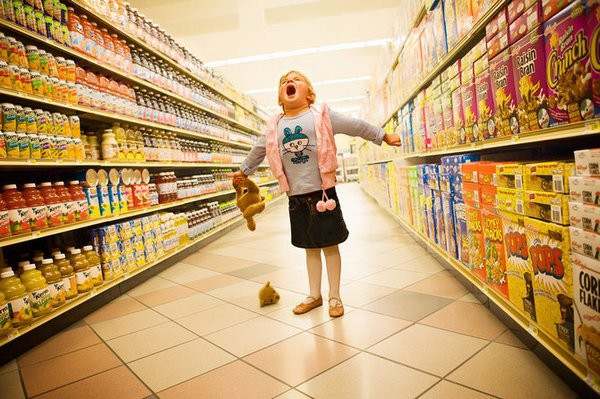
\includegraphics[width = 0.8\linewidth]{rebenok.jpeg}
            \endminipage\hfill
        \end{figure}
        }
        \visible<2>{
        \begin{figure}[t!]
            \minipage{0.6\textwidth}
              \center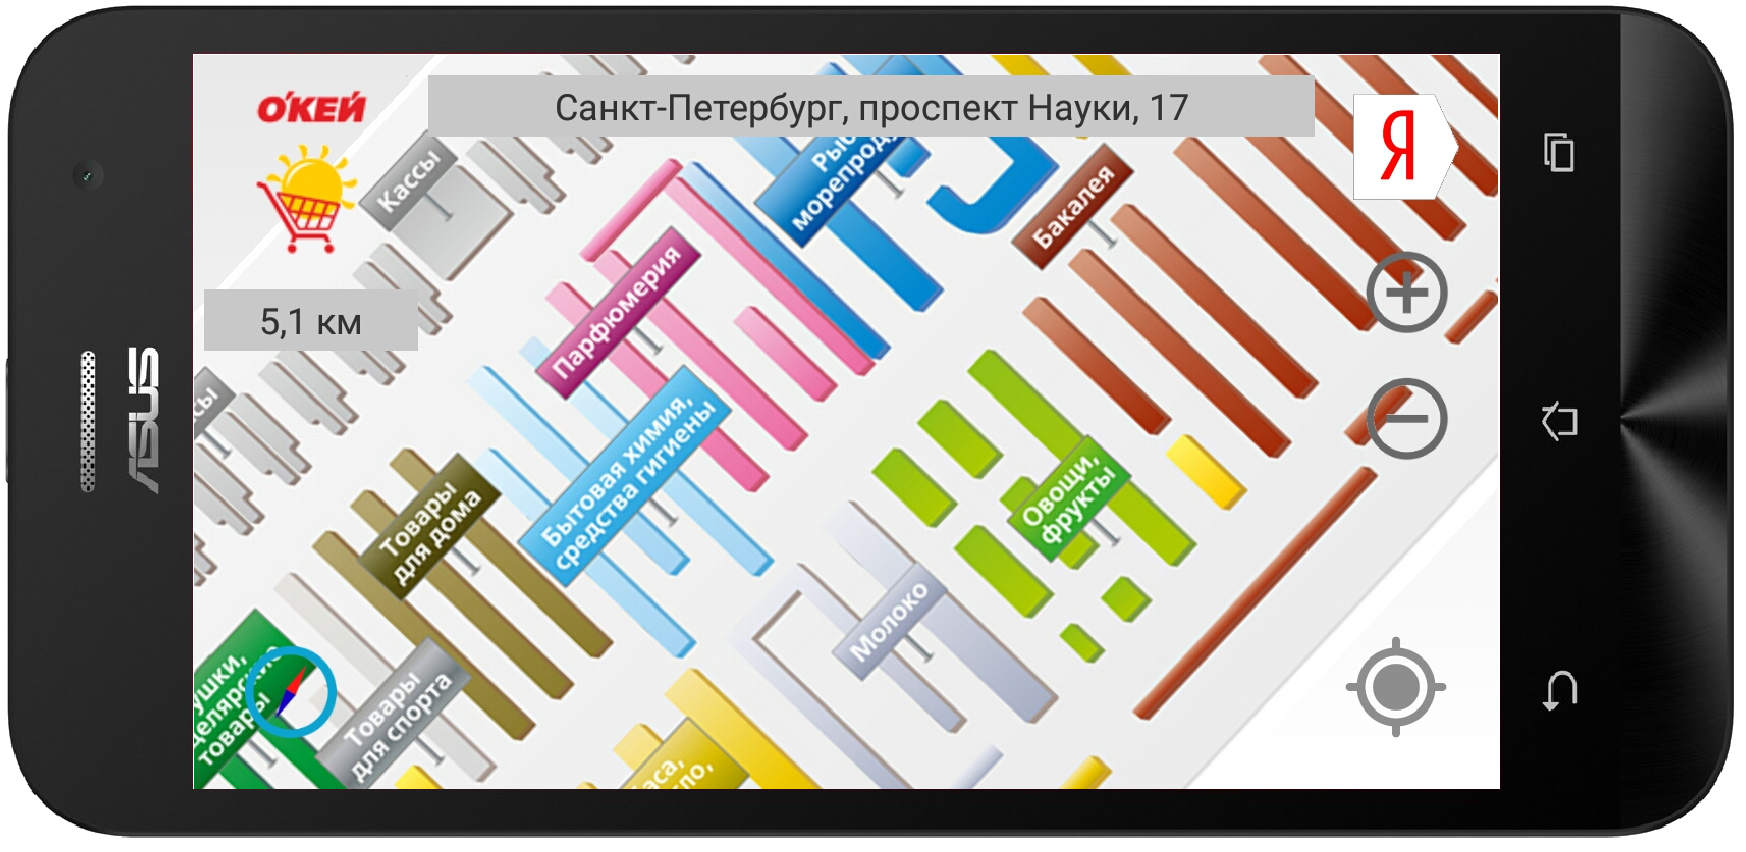
\includegraphics[width = 0.8\linewidth]{screenFirstAsus.png}
            \endminipage\hfill
            \minipage{0.4\textwidth}
              \center{Решение --- <<навигатор>> для гипермаректов}
            \endminipage\hfill
        \end{figure}
        }
    \end{figure}

	\end{frame}

    \begin{frame}
         \center\Huge\textbf{HyperNavi}
         \begin{figure}[t!]
            \begin{center}
                
\includegraphics[width =0.6\textwidth]{logo.png}

            \end{center}
       \end{figure}

    \end{frame}

    \begin{frame}{Клиент}

        \begin{figure}[t!]
            \minipage{0.5\textwidth}
              \center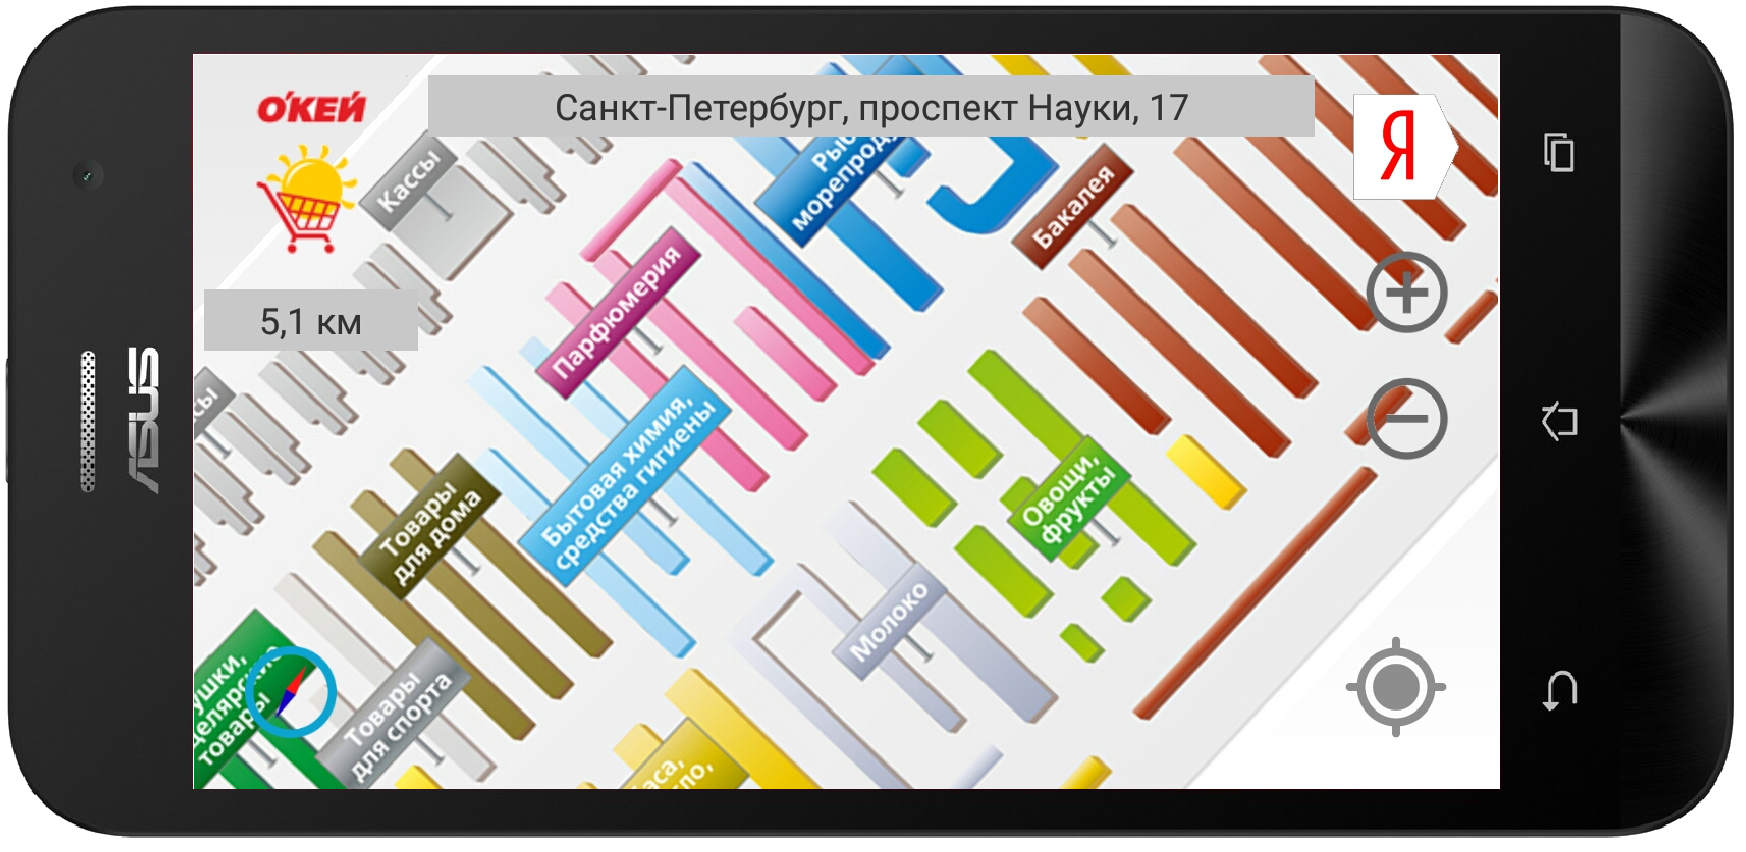
\includegraphics[width = \linewidth]{screenFirstAsus.png}
              \center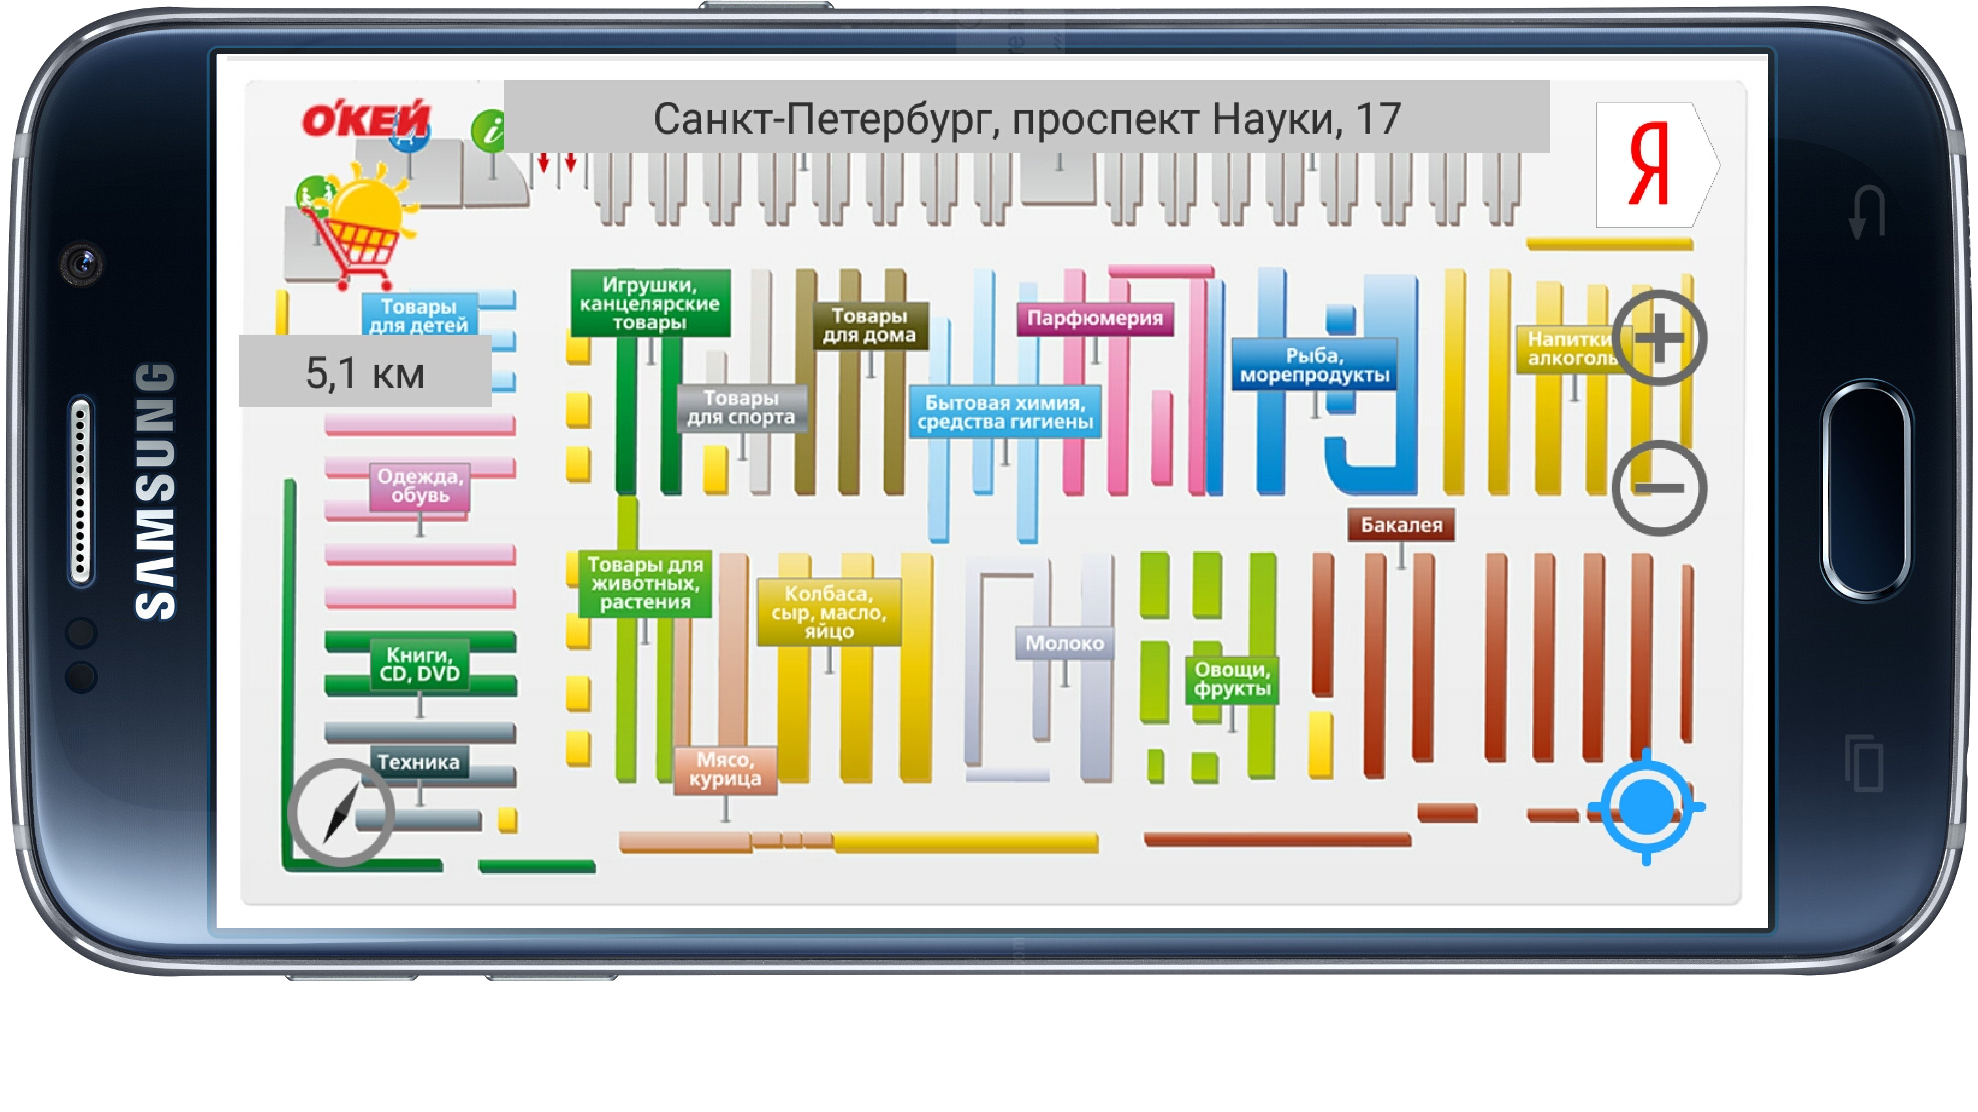
\includegraphics[width = \linewidth]{screenSecondSamsung.png}
            \endminipage\hfill
            \minipage{0.5\textwidth}
              \center
\includegraphics[width = \linewidth]{logosClient.png} %must be client_logos!
            \endminipage\hfill
        \end{figure}
    \end{frame}

    \begin{frame}{Сервер}

        \begin{figure}[t!]
            \minipage{0.5\textwidth}
              \center
\includegraphics[width = \linewidth]{logosServer.png} %must be server_logos!
            \endminipage\hfill
            \minipage{0.5\textwidth}
              \center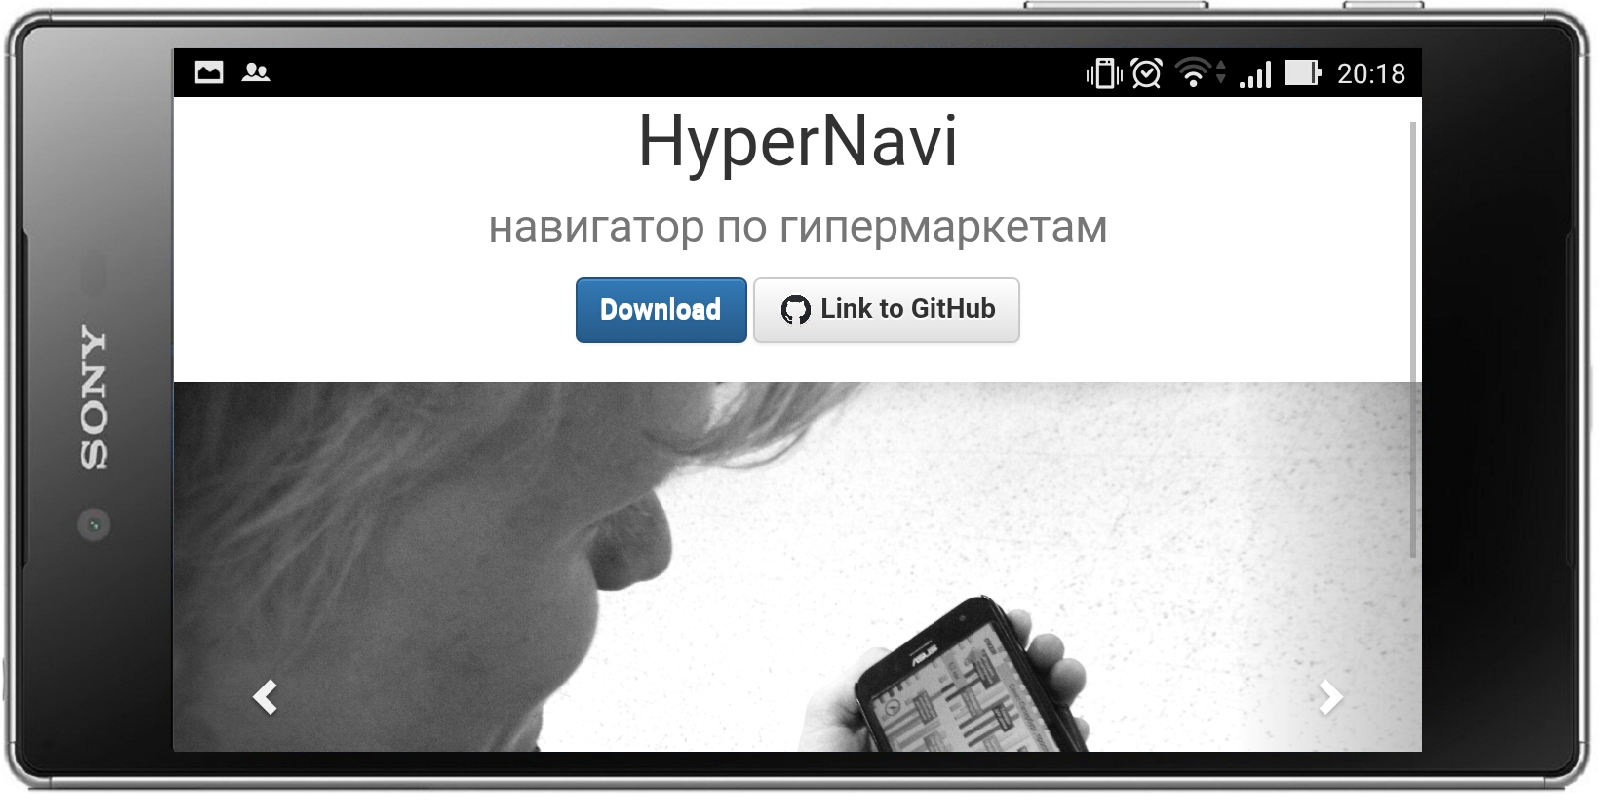
\includegraphics[width = \linewidth]{site.png}
              \center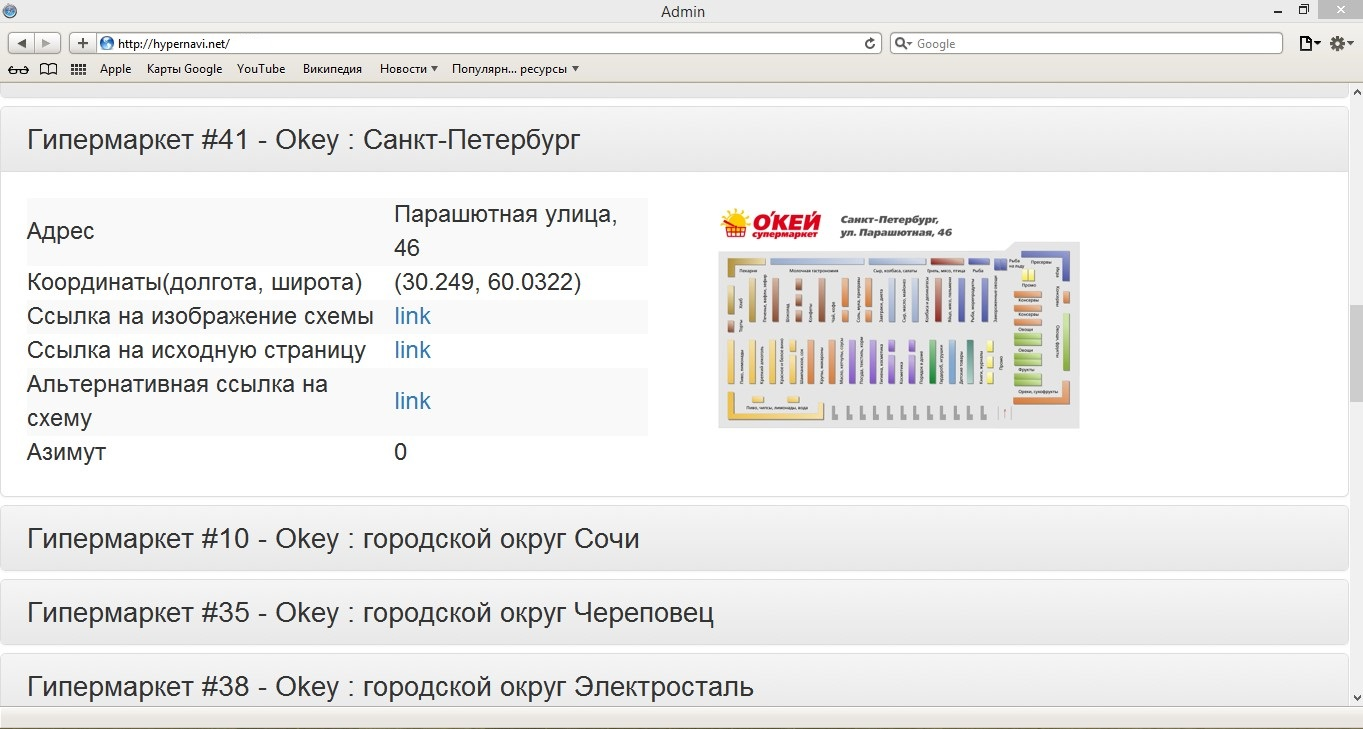
\includegraphics[width = \linewidth]{admin.jpg}
            \endminipage\hfill
        \end{figure}
    \end{frame}

    \begin{frame}{Агрегация информации}
        Для работы приложения требуются данные о гипермаркетах.
        \itemize{
         \item Имеющиеся в открытом доступе схемы гипермаркетов разбросаны по сети, разбавлены сторонней информацией.
         \item Не ясно, какая часть схем представлена.
         \item Требуется проверка актуальности информации, привязка к иным данным (координаты, адрес).
        }
    \end{frame}

    \begin{frame}{Агрегация информации}
            С помощью Weka был получен мультиклассификатор, обученный на множестве из более 100 картинок, найденных по запросу <<схема гипермаркета>>. \\
            В качестве фич были использованы следующие параметры:
            \begin{itemize}
                \item цветовые параметры схемы
                \item количество областей с текстом
                \item геометрические параметры картинок
                \item детектор границ Кенни
            \end{itemize}
    \end{frame}
    \begin{frame}{Агрегация информации}
        \begin{center}
            \begin{itemize}
                \item Классификатор был применен к картинкам с официального сайта сети гипермаркетов <<Окей>>.
                \item Были достигнуты следующие показатели: \\
                $$
                    \textnormal{precision }= 95.23 \%
                $$
                $$
                    \textnormal{recall} = 95.23 \%
                $$
                \item Наличие на каждой странице с картинкой метки на яндекс картах упростило привязку схемы к конкретному гипермаркету.
            \end{itemize}
        \end{center}
        \center{
\includegraphics[width = 1\linewidth]{logosML.png}}
    \end{frame}

    \begin{frame}{Результаты}
        \begin{itemize}
            \item Android-приложение, позволяющее в подробностях рассмотреть сориентированную карту ближайшего гипермаркета.
            \item Сервер, обрабатывающий запросы клиента.
            \item Добавлены все схемы гипермаркета <<Окей>> лежащие на официальном сайте.
            \item Мультиклассификатор схем гипермаркетов.
            \item Сайт приложения позволяющий скачать последнюю версию приложения.
        \end{itemize}
    \end{frame}

    %\begin{frame}{Клиент}
    %    \begin{figure}[h!]
    %        \center{\includegraphics[width=0.95\linewidth]{secondScreen.jpg}}
    %    \end{figure}
    %\end{frame}

    \begin{frame}{Планы}
        \begin{itemize}
            \item Увеличить базу данных:
            \begin{itemize}
                \item[•] Научиться парсить другие сайты гипермаркетов, помимо <<Окея>>.
                \item[•] Написать робота, ищущего похожие картинки и классифицирующего их.
            \end{itemize}
            \item Подумать над расширением области применения приложения (моллы, спортивные комплексы и прочее).
            \item Научиться распознавать текст на картах:
            \begin{itemize}
                \item[•] Появится функциональность поиска товаров на схеме.
                \item[•] Получать адреса из картинок.
            \end{itemize}
            \item Получать ориентацию гипермаркета в пространстве.
        \end{itemize}
    \end{frame}

    \begin{frame}
        \begin{huge}
            \begin{center}
                \vskip50pt
                Спасибо за внимание!
                \vskip0pt plus 1filll
                \large\href{http://hypernavi.net/}{http://hypernavi.net/} \\
                \vskip5pt
                \large\href{https://github.com/amosov-f/hypernavi}{https://github.com/amosov-f/hypernavi}

            \end{center}
        \end{huge}
	\end{frame}


\end{document} 